In this chapter, we give an introduction to the basic algorithms and constructions in isogeny-based cryptography.
This field began in 2006 with the ideas of Couveignes \cite{old_isogeny_crypto1}, Rostovtsev and Stolbunov \cite{old_isogeny_crypto2, old_isogeny_crypto3}, who proposed a key exchange somewhat similar to the classical Diffie-Hellman, but secure against quantum attacks.
Since then, a variety of protocols have been found, for example post-quantum key exchanges (most prominently SIDH \cite{sidh}), variants of collision resistant hash functions (most prominently the GCL hash function \cite{supersingular_hash_function}), digital signature schemes (e.g. \cite{digital_signature}) and others. 
The fundamental idea underlying all those methods is to take a random walk in an expander graph, and use that the final curve in the walk seems to be behave in an unpredictable way.

The most general problem that isogeny-based cryptography reduces to, is the \emph{explicit isogeny problem}.
\begin{problem}
    Given two Elliptic Curves $E$ and $E'$ isogeneous of fixed degree $d$, find a $d$-isogeny $\phi: E \to E'$.
\end{problem}
There are algorithms to compute such an isogeny in time polynomial in $d$, and so we usually are interested in exponentially large degrees $d$.
However, this raises the question on how to even represent the isogeny $\phi$.
In most cases, we thus require $d$ to be smooth, in which case we can represent an isogeny of degree $d$ as a sequence of small-degree isogenies.
This gives us the \emph{smooth isogeny problem}.
\begin{problem}
    Given two Elliptic Curves $E$ and $E'$ isogeneous of fixed $B$-smooth degree $d$, find a sequence of isogenies
    \begin{equation*}
        E \overset{\phi_0}{\longrightarrow} E_1 \overset{\phi_1}{\longrightarrow} \ ... \ \overset{\phi_{n - 1}}{\longrightarrow} E_n \overset{\phi_n}{\longrightarrow} E'
    \end{equation*}
    of small degree $\deg(\phi_i) \leq B$.
\end{problem}
Finally, if we further restrict the smoothness condition, and require the degree to be a power of a small prime $l$, we arrive at the \emph{isogeny path problem}.
\begin{problem}
    Given two Elliptic Curves $E, E'$ in the same connected component of $\Gamma_l(\F_q)$, find a path
    \begin{equation*}
        E \to E_1 \to ... \to E_n \to E'
    \end{equation*}
    in $\Gamma_l(\F_q)$.
\end{problem}
This problem is conjectured to be extremely hard, even for quantum computer.
Since this is in some sense the reverse problem of doing a random walk in $\Gamma_l(\F_q)$, we easily see that this gives us a one-way function.

Note that many cryptosystems use variants of above problem, e.g. similar to how classical Diffie-Hellman does not rely on the discrete logarithm problem itself, but on a (possibly easier) variant.

Finally, there is another very important problem, the \emph{endomorphism ring problem}.
\begin{problem}
    Given an Elliptic Curve $E$, find the endomorphism ring $\End(E)$.
\end{problem}
There are two possible interpretations of this:
Either we are required to compute the isomorphism type of $\End(E)$, i.e. a description of the ring structure of $\End(E)$.
In the ordinary case, this could be the discriminant $d(\End(E))$.
The stronger interpretation on the other hand would require us to compute generator isogenies of $\End(E)$, again represented as a sequence of small-degree isogenies.
It is an interesting and nontrivial fact that in the supersingular case (which is the one we are interested in), both these problems are equivalent to the isogeny path problem \cite{endomorphism_ring_isogeny_path_equivalent}.
In other words, if we know $\End(E)$ and $\End(E')$ for supersingular $E$ and $E'$, we can find an isogeny path from $E$ to $E'$.

While it is technically not a cryptosystem, we first want to present Sutherland's supersingularity test.
It is a clever algorithm based on isogeny graphs, and will be important again later.

\section{Sutherland's supersingularity test}
Consider the following problem: Given an Elliptic Curve $E$ over $\F_{p^2}$, determine whether $E$ is supersingular.
If the j-invariant $j(E) \neq 0, 1728$, one way could be to check whether $[p] = \pm \pi$ for the $p^2$-th power Frobenius endomorphism of $E$.
To do this, just sample random points $P$ and check whether $[p](P) = \pm \pi(P)$.
If this is the case for many different $P$, then $E$ is supersingular with high probability
\footnote{We also want to mention that there are more efficient probabilistic algorithms for supersingularity testing, and the above is only for illustrative purposes.}.

However, this method is only probabilistic and cannot prove that $E$ is supersingular.
In particular, in the ordinary case, the nonconstant isogeny $[p] - \pi$ can still have separability degree $O(p)$, and thus have an exponentially large kernel.

Therefore, to prove supersingularity, different methods are needed.
Sutherland \cite{sutherland_supersingularity_test} proposed the following method based on isogeny graphs.

Note that $E$ is defined over $\F_{p^2}$ if and only if there is a nontrival element of norm $p^2$ in $\End(E)$ (either this element or its conjugate must be the $p^2$-th power Frobenius).
Now assume we have an ordinary curve $E$ over $\F_{p^2}$ on the $i$-th lava flow level in the $2$-isogeny vulcano.
Then the curves on the $(i + j)$-th lava flow level have the endomorphism ring $\Z + 2^j\End(E)$ by Prop.~\ref{prop:isogeny_vulcano}.
Assuming that $\pi \in \Z + 2^j\End(E)$, we then find that
\begin{equation*}
    2^{2j} |d(\End(E))| \divides |d(\Z[\pi])| = 4p^2 - \mathrm{Tr}(\pi) \leq 4p^2
\end{equation*}
Hence $2^{2j} \leq 4p^2$, and so if
\footnote{As we will later see, this bound is not optimal. This was first noted by \cite{fp_supersingularity_tests}, and we present the optimal bound in Prop.~\ref{prop:counting_fp2_vulcano_levels}.}
$j \geq \log_2(p) + 1$, it follows that $\pi \notin \Z + 2^j\End(E)$.
In other words, if we go down $\log_2(p) + 1$ levels from $E$, we encounter a curve not defined over $\F_{p^2}$.
On the other hand, the whole supersingular 2-isogeny graph is defined over $\F_{p^2}$, so any path we take ends with a curve defined over $\F_{p^2}$.

The only obstacle to making this into a supersingularity test is that there is no way how we can ``go down'' the lava flow, i.e. we do not know which of the 2-isogenies from $E$ to one of its 2-isogeneous neighbors is the descending one.
In other words, if we just take any (non-backtracking) path starting from $E$, we might end up going around the crater of the 2-isogeny vulcano, and not down the lava flow.
Sutherland's idea now is to simultaneously take three different (non-backtracking) random walks from $E$, but ensure that they have different second vertices.
Hence, one of them will go down one step in the lava flow, and since the lava flow consists of trees, continue to go downwards.
This yields Algorithm~\ref{alg:sutherland_supersingularity_test}.
\begin{algorithm}
\caption{\label{alg:sutherland_supersingularity_test} Sutherland's supersingularity test\\
\textbf{Input:} A j-invariant $j_0$\\
\textbf{Output:} True if the isomorphism class of curves represented by $j$ is supersingular}
\begin{algorithmic}[1]
\State Compute the modular polynomial $\Phi_2$
\State Set $j_0^{(0)} = j_0^{(1)} = j_0^{(2)} = j_0$
\State Set $j_1^{(0)}, j_1^{(1)}, j_1^{(2)}$ to the three roots of $\Phi_2(X, j_0)$
\For{$k \in \{0, 1, 2\}$}
    \For{$i = 1$ to $\lfloor \log_2(p) \rfloor$}
        \State Set $j_{i + 1}^{(k)}$ to any root of $\Phi_2(X, j_i^{(k)})$ other than $j_{i - 1}^{(k)}$
        \If{$j_{i + 1}^{(k)} \notin \F_{p^2}$}
            \Return False
        \EndIf
    \EndFor
\EndFor
\State \Return True
\end{algorithmic}
\end{algorithm}

Variants of Sutherland's supersingularity test are still the best deterministic general-purpose supersingularity check.
In particular, they are faster than ideas based on point counting.
Hence, this algorithm also plays an important role in isogeny-based cryptography, e.g. for key validation.

\section{Supersingular Isogeny Diffie-Hellman}
Even though the Supersingular Isogeny Diffie-Hellman (SIDH) scheme is broken, we think its ideas are important and serve well to illustrate the basic approach in isogeny-based cryptography.
Hence, we want to given an overview in this section.

The basic structure of SIDH is, as the name suggests, somewhat similar to the classical Diffie-Hellman key exchange.
The basic idea is that both Alice and Bob take a random walk start from a joint curve $E$ in the supersingular $l_A$-resp. $l_B$-isogeny graph, ending at curves $E_A$ and $E_B$.
Now they exchange these curves, and then take the ``same'' walk on the other curve, i.e. Alice performs the same walk again, but this time starting from $E_B$ and similar for Bob.
Hence, Alice ends up at a curve $E_{BA}$ and Bob with a curve $E_{AB}$.
We want that $E_{AB} \cong E_{BA}$, and then $j(E_{AB}) = j(E_{BA})$ can be used as a shared secret key.

However, to achieve this, we need a suitable notion of the ``same'' walk, starting from a different curve.
The way to achieve this in SIDH is to share some additional information about the isogenies $E \to E_A$ resp. $E \to E_B$.

More concretely, Alice's isogeny $\phi_A: E \to E_A$ is determined by a cyclic subgroup of $E[l_A^{e_A}]$, thus has a generator point $A \in E[l_A^{e_A}]$.
Since $E[l_A^{e_A}] \cong (\Z/l_A^{e_A}\Z)^2$, it has a $(\Z/l_A^{e_A}\Z)$-basis, say $P_A$ and $Q_A$.
Now $A = m_A P_A + n_A Q_A$, and similarly, we have for Bob that $B = m_B P_B + n_B Q_B$ where $P_B$ and $Q_B$ are a basis of $E[l_B^{e_B}]$.
After both Alice and Bob exchange their curves $E_A$ and $E_B$, they also publish the additional points $\phi_A(P_B), \phi_A(Q_B), \phi_B(P_A), \phi_B(Q_A)$.
This now allows Alice to take the $l_A^{e_A}$-isogeny from $E_B$ with kernel generated by $m_A \phi_B(P_A) + n_A \phi_B(Q_A)$.
In other words, the notion of the ``same'' walk refers to the corresponding isogenies having the same kernel under the isomorphism
\begin{equation*}
    E[l_A^{e_A}] \overset{\sim}{\longrightarrow} E_B[l_A^{e_A}], \quad P \mapsto \phi_B(P)
\end{equation*}
Now it is not hard to show that this commutes in an appropriate sense, i.e. $E_{AB} \cong E_{BA}$.
This method is also displayed in Figure~\ref{fig:sidh}.
\begin{figure}
    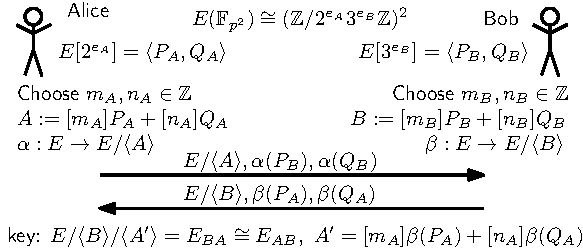
\includegraphics[width = \textwidth]{./sidh.pdf}
    \caption{\label{fig:sidh} The SIDH protocol for $l_A = 2$ and $l_B = 3$.}
\end{figure}

Note that these additional published points $\phi_A(P_B), \phi_A(Q_B), \phi_B(P_A), \phi_B(Q_A)$ make the security assumption required for SIDH somewhat nonstandard.
In particular, it is not enough to assume that the isogeny path problem is hard, and also if we relax this in an analogeous way to the classical Diffie-Hellman assumption (i.e. it is impossible to find $E_{AB}$ given $E_A$ and $E_B$) is not enough.
As it turns out, this additional information indeed decreases the security, as first mentioned by Cristophe Petit \cite{torsion_point_attack}.
However, it still was a big shock when \cite{sidh_broken} discovered an efficient attack using these torsion points, bringing the complete demise of SIDH.
This is even more surprising, as an SIDH-based cryptosystem named SIKE \cite{sike} was already considered a promising candidate for post-quantum crypto, and made it into the fourth (and final) round of the NIST post-quantum standardization process.

Since SIDH is broken, it does not serve perfectly to motivate the usefulness of a way to generate supersingular curves without revealing a trapdoor.
Still, we want to mention that choosing a starting curve with unknown endomorphism ring can prevent the torsion point attacks of \cite{torsion_point_attack}.
Next, we want to present another, slightly more exotic cryptosystem for which it is important to have a hard starting curve, i.e. a curve for which nobody knows a trapdoor (e.g. the endomorphism ring).

\section{An isogeny-based verifiable delay function}
\label{sec:verifiable_delay_function}
In this section, we present the verifiable delay function by De Feo, Masson, Petit and Sanso \cite{verifiable_delay_function}.
A \emph{verifiable delay function} (VDF) as first formalized in \cite{definition_verifiable_delay_function} is a cryptographic primitive consisting of three algorithms
\begin{itemize}
    \item \textbf{KeyGen}$(\lambda, T)$ takes a security parameter $\lambda$ and a time parameter $T$ and computes a pair $(\mathrm{ek}, \mathrm{vk})$ of an evaluation key $\mathrm{ek}$ and a verification key $\mathrm{vk}$.
    \item \textbf{Eval}$(\mathrm{ek}, s)$ takes the evaluation key and an input $s$ and computes an output $a$. 
    The key feature is that it should be impossible to compute \textbf{Eval} in time less than $T$, no matter how much parallel computing capabilities are available.
    \item \textbf{Verify}$(\mathrm{vk}, s, a)$ takes the verification key, the input $s$ and the output $a$ and checks whether \textbf{Eval}$(\mathrm{ek}, s) = a$.
\end{itemize}
Both \textbf{KeyGen} and \textbf{Verify} should run in time $O(\mathrm{poly}(\lambda))$, while \textbf{Eval} should (of course) run in time $T$.
The security of the VDF consists then of the three properties \emph{Correctness}, \emph{Soundness} and \emph{Sequentiality}.
As usual, correctness and soundness refer to the fact that \textbf{Verify} accepts correctly computed outputs (i.e. by \textbf{Eval}) and declines other outputs, both with probability $1 - 2^{-\lambda}$.
The interesting property is sequentiality, which states that it is impossible to compute \textbf{Eval}$(\mathrm{ek}, s)$ in less than $T$ computational steps, no matter how much parallel processing is available.

Therefore, a verifiable delay function provides a way of ensuring that an output $a$ is only known after a certain amount of wall clock time has elapsed (starting from the point at which the input $s$ is known).
Most applications focus on the use to generate public, trusted randomness: Some public entropy source provides the input $s$, but we assume that an attacker has ways to influence the entropy source (a common example are stock market prices).
To prevent an attacker from exploiting this, one now uses the entropy source $a = $ \textbf{Eval}$(\mathrm{ek}, s)$ instead, which can still be manipulated by the attacker, but not exploited anymore.
More concretely, if $T$ is larger than the natural change interval of the source $s$, an attacker cannot predict fast enough how a manipulation influences the output, and thus not profit from it.
There are more applications, for example in blockchain technology.

The isogeny-based VDF from \cite{verifiable_delay_function} relaxes this slightly by allowing the setup routine to take time $O(\mathrm{poly}(\lambda, T))$.
Apart from that, it satisfies above security properties under some isogeny-related security assumptions.
The basic idea is as follows.

The only efficient way we know to evaluate an isogeny $\psi: E \to E'$ of exponential degree $l^T$ is to write it as a sequence
\begin{equation*}
    E = E_0 \overset{\psi_1}{\longrightarrow} E_1 \overset{\psi_2}{\longrightarrow} \ ... \ \overset{\psi_T}{\longrightarrow} E_T = E'
\end{equation*}
of $l$-isogenies, and then compute the points $P_i = \psi_i(P_{i - 1})$ for an input point $P_0 \in E$.
Clearly, since $P_i$ depends on $P_{i - 1}$, it is impossible to effectively parallelize that.
Hence, it seems like a reasonable security assumption that $\psi(P)$ cannot be evaluated in less than $T$ time steps, and thus can be used for the function \textbf{Eval}.

Verification on the other hand can now be done using the Weil pairing.
If $P \in E[m]$ (with $m$ coprime to $l$ and $p$), we have that
\begin{equation*}
    e_m(\hat{\psi}(P), Q) = e_m(P, \psi(Q))
\end{equation*}
and (assuming that $\hat{\psi}(P)$ is known), we can compute $e_m(\hat{\psi}(P), Q)$ very efficiently.
There is just one problem here.
The map $e_m(P, \cdot): E[m] \to \mu_m$ obviously cannot be injective by a cardinality argument, and indeed, given $\psi(Q)$ we can easily compute other points $Q'$ with
\begin{equation*}
    e_m(P, \psi(Q)) = e_m(P, Q')
\end{equation*}
This obviously violates the soundness of system, as an attacker could compute $Q = $ \textbf{Eval}$(\mathrm{ek}, Q) = \psi(Q)$, but then claim $Q'$ to be the result.
Verification as above will not detect this.
To make it work, \cite{verifiable_delay_function} proposes to assume that $E/\F_p$ and use the trace map
\begin{equation*}
    \mathrm{Tr}: E[m] \to E[m] \cap E(\F_p), \quad P \mapsto P + \pi_E(P)
\end{equation*}
This map is $m$-to-1, and we have that
\begin{equation*}
    e_m(P, \mathrm{Tr}(\psi(Q))) = e_m(\hat{\psi}(P), Q)^2
\end{equation*}
which can be used for verification.
This now works, since the map $e_m(P, \cdot): E[m] \cap E(\F_p) \to \mu_m$ is indeed bijective for suitable choices of $P$.
Therefore, we get the scheme displayed in Algorithms~\ref{alg:setup_vdf}, \ref{alg:eval_vdf} and~\ref{alg:verify_vdf}.
\begin{algorithm}
    \caption{\label{alg:setup_vdf} \textbf{Setup}\\
    \textbf{Input:} A security parameter $\lambda$ and a time parameter $T$\\
    \textbf{Output:} Curves $E$ and $E'$, an evaluation key $\psi: E' \to E$ and a verification key $(P, \hat{\psi}(P))$}
    \begin{algorithmic}[1]
        \State Find distinct primes $p$ and $m$ of size depending on $\lambda$
        \State Find a random supersingular Elliptic Curve $E$ over $\F_p$
        \State Take a random walk of length $T$ starting from $E$ in the 2-isogeny graph, given by $\hat{\psi}: E \to E'$
        \State Find a random point $P \in E[m]$
        \State Compute $\hat{\psi}(P)$
        \State\Return $\mathrm{ek} = (E, E', \psi)$ and $\mathrm{vk} = (E, E', P, \hat{\psi}(P))$
    \end{algorithmic}
\end{algorithm}
\begin{algorithm}
    \caption{\label{alg:eval_vdf} \textbf{Eval}\\
    \textbf{Input:} The evaluation key $(E, E', \psi)$ and an input point $Q \in E'[m]$\\
    \textbf{Output:} An output point $Q' \in E[m]$}
    \begin{algorithmic}[1]
        \State Compute $\psi(Q)$
        \State\Return $Q' := \mathrm{Tr}(\psi(Q))$
    \end{algorithmic}
\end{algorithm}
\begin{algorithm}
    \caption{\label{alg:verify_vdf} \textbf{Verify}\\
    \textbf{Input:} The verification key $(E, E', P, \hat{\psi}(P))$, an input $Q \in E'[m]$ and an output $Q'$\\
    \textbf{Output:} An output point $\psi(Q)$}
    \begin{algorithmic}[1]
        \If{$Q' \in \mathrm{im}(\mathrm{Tr}) = E[m] \cap E(\F_p)$ and $e_m(P, Q') = e_m(\hat{\psi}(P), Q)^2$}
            \State\Return Valid
        \Else
            \State\Return Invalid
        \EndIf
    \end{algorithmic}
\end{algorithm}

In a practical implementation, we might want to exclude $P \in E[m]$ such that the map $e_m(P, \cdot): E[m] \cap E(\F_p) \to \mu_m$ is not bijective.
This is done in \cite{verifiable_delay_function}, but we will ignore those cases here.
Furthermore, we also will not prove that this is indeed a VDL, again refering the reader to \cite{verifiable_delay_function}.

However, we do want to discuss step 2 in the setup step, Algorithm~\ref{alg:setup_vdf}.
In particular, we claim that the curve $E$ has to be generated in a way that does not reveal its endomorphism ring $\End(E)$, or the resulting scheme will be insecure.
Hence, the classical methods of using CM techniques and random walks fail here.
Since there is currently no known alternative, at the moment this VDF requires a trusted party to generate the cuve $E$, and then forget about its endomorphism ring.

Namely, note that breaking sequentiality of the VDF can be achieved by solving the \emph{isogeny shortcut problem}.
\begin{problem}
    Given an isogeny $\psi: E \to E'$ of exponential degree $l^T$ and a point $Q \in E$, compute $\psi(Q)$ in time less than $T$.
\end{problem}
Since the supersingular isogeny graph is an expander, there exists always a path $E \to E'$ of length $O(\log(p))$.
Hence, if $T \in \omega(\log(p))$, we can solve the isogeny shortcut problem by the following three steps
\begin{itemize}
    \item Find an isogeny $\phi: E \to E'$ of degree at most $l^{O(\log(p))}$
    \item Find an endomorphism $\alpha \in \End(E')$ such that $\restr{\alpha \circ \phi}{E[m]} = \restr{\psi}{E[m]}$
    \item Evaluate $\alpha(\phi(P))$
\end{itemize}
Using similar techniques to the reductions between the isogeny path problem and the endomorphism ring problem \cite{endomorphism_ring_isogeny_path_equivalent}, the authors in \cite{verifiable_delay_function} have now shown that all three of these steps are indeed possible in time polynomial in $\log(T)$ if the endomorphism ring $\End(E)$ is known.
Hence, anyone who knows the endomorphism ring of the starting curve $E$ from Algorithm~\ref{alg:setup_vdf} can compute \textbf{Eval} in time less than $T$, thus breaking the protocol.

This is one of several examples why the generation of supersingular curves without revealing a trapdoor would be an important tool for cryptography.
However, as already mentioned, it is still an open problem to find an algorithm that achieves this.
In the next chapter, we will now present the progress we made on this problem. 